\documentclass[tikz,border=2pt]{standalone}
\usepackage{amsmath,amssymb}
\usepackage{tikz}

\begin{document}
% Two different spanning trees of the same network: each keeps all 6 vertices and 5 of the
% 9 edges, forming a tree.
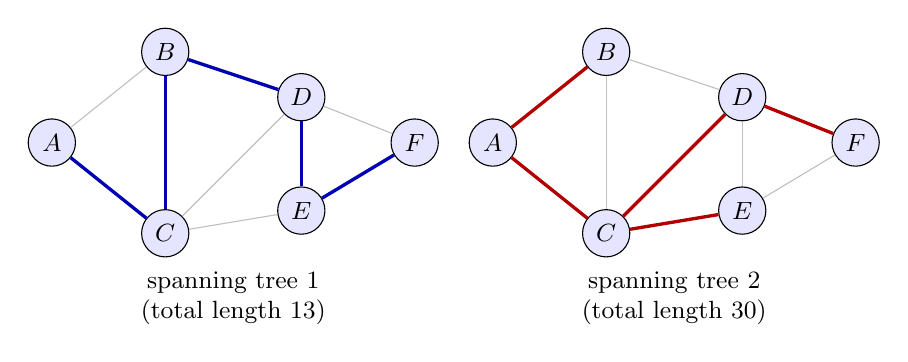
\begin{tikzpicture}[every node/.style={font=\small}, v/.style={draw, circle, fill=blue!10, minimum size=6mm, inner sep=0pt}]
	\begin{scope}[x=0.72cm, y=0.72cm]
		\node[v] (A) at (0,0) {$A$}; \node[v] (B) at (2,1.6) {$B$}; \node[v] (C) at (2,-1.6) {$C$}; \node[v] (D) at (4.4,0.8) {$D$}; \node[v] (E) at (4.4,-1.2) {$E$}; \node[v] (F) at (6.4,0) {$F$};
		\foreach \a/\b in {A/B, A/C, B/C, B/D, C/D, C/E, D/E, D/F, E/F} {\draw[gray!50] (\a) -- (\b);}
		\foreach \a/\b in {A/C, C/B, B/D, D/E, E/F} {\draw[blue!70!black, very thick] (\a) -- (\b);}
		\node[anchor=north, align=center] at (3.2,-2.1) {spanning tree 1\\ (total length $13$)};
	\end{scope}
	\begin{scope}[x=0.72cm, y=0.72cm, xshift=5.6cm]
		\node[v] (A) at (0,0) {$A$}; \node[v] (B) at (2,1.6) {$B$}; \node[v] (C) at (2,-1.6) {$C$}; \node[v] (D) at (4.4,0.8) {$D$}; \node[v] (E) at (4.4,-1.2) {$E$}; \node[v] (F) at (6.4,0) {$F$};
		\foreach \a/\b in {A/B, A/C, B/C, B/D, C/D, C/E, D/E, D/F, E/F} {\draw[gray!50] (\a) -- (\b);}
		\foreach \a/\b in {A/B, A/C, C/E, C/D, D/F} {\draw[red!70!black, very thick] (\a) -- (\b);}
		\node[anchor=north, align=center] at (3.2,-2.1) {spanning tree 2\\ (total length $30$)};
	\end{scope}
	\end{tikzpicture}
\end{document}
